\chapter{Aplicación y validación: caso de estudio}

\section{Descripción del caso de estudio y aplicación metodológica}

El caso de estudio fue desarrollado en una institución bancaria mediana
peruana en proceso de modernización de sus canales digitales. La institución
contaba con una plataforma web desarrollada en tecnología legacy
(JSP/Struts) con más de doce años de antigüedad, cuya renovación fue
declarada prioridad estratégica por la Gerencia de Tecnología. El equipo
técnico estaba conformado por 20 profesionales --programadores, analistas
de QA y analistas funcionales-- organizados en equipos de trabajo bajo la
metodología Scrum, con distintos niveles de experiencia en tecnologías
modernas de desarrollo de interfaz de usuario y con adopción incipiente de
asistentes de código basados en IA (GitHub Copilot) en el 60\% del equipo.

La selección del caso respondió a criterios de representatividad sectorial: la
institución opera bajo la regulación de la Superintendencia de Banca, Seguros
y AFP (SBS), gestiona cerca de medio millón de cuentas activas y experimenta
picos de tráfico de hasta 15 veces el volumen base durante campañas de
captación y cierres de mes. Esta combinación de restricciones regulatorias,
complejidad arquitectónica y presión de modernización la convierte en un
caso representativo del problema central estudiado en esta investigación.

La Figura \ref{fig:4.1} presenta el diagrama del proceso de aplicación de la
metodología en el caso de estudio, detallando las actividades ejecutadas en
cada fase y los puntos de validación intermedios.

La Fase 1 (Análisis de Requisitos) requirió dos semanas e involucró
entrevistas con 12 líderes técnicos y tres oficiales de cumplimiento
regulatorio. Se identificaron 47 requisitos funcionales y no funcionales, de
los cuales 18 eran específicos del contexto bancario. La Fase 2 (Evaluación
Técnica) se extendió dos semanas adicionales, durante las cuales se
desarrollaron prototipos de concepto (\emph{Proof of Concept}) en los tres
frameworks --generados parcialmente con asistencia de IA-- para validar
aspectos críticos de integración con los sistemas core de la institución y
evaluar la consistencia del código sugerido por los asistentes.

\begin{figure}[htbp]
\centering
\begin{tikzpicture}[
  node distance=8mm and 8mm,
  box/.style={rectangle, draw, rounded corners, align=center, text width=6.2cm, minimum height=9mm, font=\small},
  phase/.style={rectangle, draw, thick, align=center, text width=6.2cm, minimum height=11mm, font=\small, fill=gray!10},
  decision/.style={diamond, draw, aspect=3, align=center, inner sep=1pt, font=\small},
  term/.style={rectangle, rounded corners=8pt, draw, thick, align=center, minimum width=2.5cm, font=\small},
  arr/.style={-{Stealth[length=2mm]}}
]
\node[term] (inicio) {INICIO};
\node[box, below=of inicio] (perfil) {Definir perfil institucional y alcance de evaluación};
\node[box, below=of perfil] (candidatos) {Identificar frameworks candidatos: Angular, React y Vue.js};
\node[phase, below=of candidatos] (f1) {FASE 1: Análisis de Requisitos\\\footnotesize Técnicos $\cdot$ Regulatorios};
\node[decision, below=10mm of f1] (d1) {\shortstack{¿Requisitos\\completos?}};
\node[phase, below=10mm of d1] (f2) {FASE 2: Evaluación Técnica\\\footnotesize Benchmarking $\cdot$ Seguridad $\cdot$ Calidad de código IA};
\node[phase, below=of f2] (f3) {FASE 3: Evaluación Regulatoria\\\footnotesize Cumplimiento $\cdot$ Gobernanza de IA $\cdot$ TCO};
\node[phase, below=of f3] (f4) {FASE 4: Decisión Final\\\footnotesize Consolidación de evaluaciones $\cdot$ Deliberación de stakeholders};
\node[decision, below=10mm of f4] (d2) {\shortstack{¿Consenso\\alcanzado?}};
\node[box, below=10mm of d2] (seleccion) {Selección formal y documentación del framework elegido};
\node[term, below=of seleccion] (fin) {FIN};

\draw[arr] (inicio) -- (perfil);
\draw[arr] (perfil) -- (candidatos);
\draw[arr] (candidatos) -- (f1);
\draw[arr] (f1) -- (d1);
\draw[arr] (d1) -- node[right,font=\scriptsize]{sí} (f2);
\draw[arr] (d1.west) -- ++(-2.3,0) -- node[left,font=\scriptsize]{no} ++(0,2.6) -- (f1.west);
\draw[arr] (f2) -- (f3);
\draw[arr] (f3) -- (f4);
\draw[arr] (f4) -- (d2);
\draw[arr] (d2) -- node[right,font=\scriptsize]{sí} (seleccion);
\draw[arr] (d2.west) -- ++(-2.3,0) -- node[left,font=\scriptsize]{no} ++(0,4.4) -- (f4.west);
\draw[arr] (seleccion) -- (fin);
\end{tikzpicture}
\caption{Proceso de aplicación metodológica en el caso de estudio (modelo técnico-regulatorio)}
\label{fig:4.1}
\end{figure}

\section{Resultados de la evaluación y decisión final}

\subsection{Puntuaciones de la evaluación técnica y regulatoria}

La aplicación sistemática de la metodología propuesta produjo las
puntuaciones ponderadas que se presentan en la Tabla \ref{tab:4.1}, sobre la
base de los diez criterios técnicos y regulatorios definidos en el Capítulo
3 (incluidos los dos criterios emergentes asociados a la IA generativa). Las
calificaciones fueron asignadas mediante consenso del Comité Evaluador,
conformado por cinco expertos de la institución: el Arquitecto Principal, el
Jefe de Seguridad (CISO), el Líder Técnico de Interfaz de Usuario, el
Oficial de Cumplimiento Regulatorio y el responsable de gobernanza de datos
e IA.

\begin{table}[htbp]
\centering
\caption{Resultados de la evaluación ponderada de frameworks en el caso de estudio}
\label{tab:4.1}
\small
\begin{tabular}{@{}p{4.6cm}p{1.2cm}ccc@{}}
\toprule
Criterio & Peso ($w_i$) & Angular & React & Vue.js \\
\midrule
Seguridad y protección              & 0.16 & 9.2  & 7.8  & 7.5 \\
Rendimiento y escalabilidad         & 0.13 & 8.5  & 8.8  & 8.0 \\
Mantenibilidad del código           & 0.13 & 9.0  & 7.5  & 7.8 \\
Calidad del código generado por IA  & 0.08 & 9.0  & 7.0  & 7.5 \\
Accesibilidad (WCAG 2.2)            & 0.06 & 8.5  & 8.0  & 8.2 \\
Compatibilidad multiplataforma      & 0.04 & 8.0  & 8.5  & 8.0 \\
Cumplimiento regulatorio            & 0.16 & 9.0  & 7.5  & 7.0 \\
Integración con sistemas legacy     & 0.12 & 8.8  & 7.8  & 7.2 \\
Alta disponibilidad (SLA)           & 0.06 & 8.7  & 8.2  & 7.8 \\
Gobernanza regulatoria del uso de IA & 0.06 & 8.8  & 7.6  & 7.3 \\
\midrule
\textbf{Puntuación ponderada total ($S_f$)} & & \textbf{8.84} & \textbf{7.83} & \textbf{7.56} \\
\bottomrule
\end{tabular}
\end{table}

\subsection{Análisis de resultados y decisión institucional}

Angular obtuvo la puntuación ponderada más alta con $S_{\text{Angular}} =
8.84$, seguido de React ($S_{\text{React}} = 7.83$) y Vue.js ($S_{\text{Vue}}
= 7.56$). La diferencia más significativa se registró en los criterios
regulatorios y de seguridad, donde Angular presentó ventajas consistentes
derivadas de su arquitectura TypeScript obligatoria y sus mecanismos nativos
de sanitización del DOM, que reducen la exposición a vulnerabilidades XSS en
interfaces bancarias complejas.

El Comité Evaluador prestó especial atención a los dos criterios emergentes.
En \emph{calidad del código generado por IA}, Angular obtuvo la calificación
más alta (9.0 frente a 7.0 de React) porque su arquitectura opinionada y su
tipado estático obligatorio redujeron en las pruebas de concepto la
variabilidad de las sugerencias de GitHub Copilot, facilitando su revisión
por el equipo técnico. En \emph{gobernanza regulatoria del uso de IA},
Angular también lideró (8.8 frente a 7.6 de React), en la medida en que su
estructura modular facilitó documentar la procedencia del código
IA-asistido ante el Oficial de Cumplimiento --un requisito que el panel de
expertos anticipa exigible en próximas actualizaciones normativas de la SBS.
React demostró ventajas en rendimiento y compatibilidad multiplataforma
--criterios con pesos de 0.13 y 0.04, respectivamente-- lo que generó debate
en el Comité Evaluador durante la Fase 4, pero la ponderación mayor de los
criterios de seguridad, cumplimiento e integración legacy inclinó la
decisión hacia Angular.

Vue.js fue descartado en etapas intermedias de la evaluación principalmente
por sus calificaciones más bajas en cumplimiento regulatorio y en
gobernanza de IA, asociadas a una comunidad de práctica más pequeña en
torno a herramientas de auditoría de código IA-asistido para este
framework.

La institución bancaria seleccionó formalmente Angular como tecnología
de interfaz de usuario para su plataforma de canales digitales. La decisión fue
documentada y aprobada por el Comité de Arquitectura Tecnológica en sesión
formal, con todas las justificaciones trazables a los resultados de
evaluación. El plan de adopción contempló un período de migración gradual de
18 meses estructurado en tres etapas: piloto funcional (meses 1--4),
migración modular por dominio de negocio (meses 5--14) y cierre de la
plataforma legacy (meses 15--18).

\subsection{Análisis gráfico de los resultados}

La Figura \ref{fig:4.2} resume las puntuaciones globales $S_f$ y la Figura
\ref{fig:4.3} descompone el rendimiento de cada framework por dimensión de
evaluación, evidenciando la ventaja diferencial de Angular tanto en el eje
técnico como en el regulatorio.

\begin{figure}[htbp]
\centering
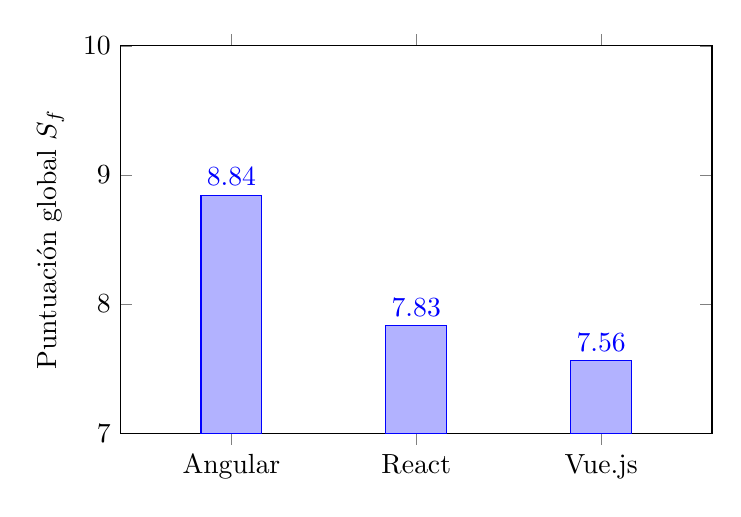
\begin{tikzpicture}
\begin{axis}[
  ybar, bar width=22pt,
  ymin=7, ymax=10,
  symbolic x coords={Angular,React,Vue.js},
  xtick=data,
  ylabel={Puntuación global $S_f$},
  nodes near coords,
  width=0.75\textwidth, height=6.5cm,
  enlarge x limits=0.3,
]
\addplot coordinates {(Angular,8.84) (React,7.83) (Vue.js,7.56)};
\end{axis}
\end{tikzpicture}
\caption{Puntuaciones ponderadas globales $S_f$ de los tres frameworks en el caso de estudio (modelo técnico-regulatorio)}
\label{fig:4.2}
\end{figure}

\begin{figure}[htbp]
\centering
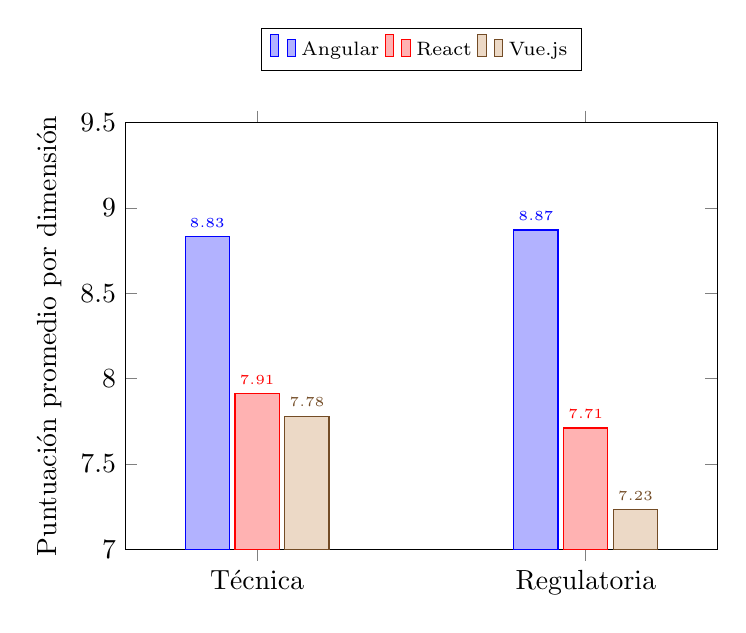
\begin{tikzpicture}
\begin{axis}[
  ybar, bar width=16pt,
  ymin=7, ymax=9.5,
  symbolic x coords={Técnica,Regulatoria},
  xtick=data,
  ylabel={Puntuación promedio por dimensión},
  legend style={at={(0.5,1.12)},anchor=south,legend columns=-1,font=\scriptsize},
  width=0.75\textwidth, height=7cm,
  enlarge x limits=0.4,
  nodes near coords, every node near coord/.append style={font=\tiny, /pgf/number format/.cd, fixed, precision=2},
]
\addplot coordinates {(Técnica,8.83) (Regulatoria,8.87)};
\addplot coordinates {(Técnica,7.91) (Regulatoria,7.71)};
\addplot coordinates {(Técnica,7.78) (Regulatoria,7.23)};
\legend{Angular,React,Vue.js}
\end{axis}
\end{tikzpicture}
\caption{Comparación de frameworks por dimensión: técnica (60\% del peso) y regulatoria (40\%). Promedios ponderados calculados a partir de la Tabla \ref{tab:4.1}.}
\label{fig:4.3}
\end{figure}

\subsection{Análisis de sensibilidad de los pesos AHP}

El AHP produce resultados condicionados a los pesos consensuados por el
panel Delphi. Un análisis de sensibilidad verifica si la elección de Angular
se mantiene ante redistribuciones razonables de esos pesos, descartando que
el resultado sea un artefacto de la ponderación específica obtenida (Saaty,
1980). Los puntajes por criterio ($r_{fi}$) se mantienen fijos en los valores
de la Tabla \ref{tab:4.1}; únicamente varían los $w_i$.

Se diseñaron cinco escenarios alternativos (S1--S5). Los escenarios S1 y S2
redistribuyen el peso entre las dimensiones técnica y regulatoria
manteniendo ambas dentro del modelo. El escenario S3 es el más relevante
para la Hipótesis Específica 6 (sección 1.4.2): recalcula la decisión
\textbf{excluyendo por completo los dos criterios asociados a la IA
generativa} y redistribuyendo proporcionalmente su peso (14\%) entre los
ocho criterios restantes, para aislar el efecto neto de haber incorporado
la IA generativa al modelo. El escenario S4 asigna peso uniforme a los diez
criterios. El escenario S5 representa un límite teórico extremo,
concentrando el 100\% del peso en los dos únicos criterios donde React
supera a Angular (rendimiento y compatibilidad) e ignorando por completo
seguridad y cumplimiento normativo --una configuración inviable en un banco
regulado, incluida únicamente para acotar el dominio de robustez del
modelo.

\begin{table}[htbp]
\centering
\caption{Análisis de sensibilidad: puntuaciones $S_f$ ante variaciones en los pesos AHP. Los $r_{fi}$ permanecen fijos en los valores de la Tabla \ref{tab:4.1}.}
\label{tab:4.2}
\small
\begin{tabular}{@{}cp{6cm}cccc@{}}
\toprule
Esc. & Descripción de la redistribución & Angular & React & Vue.js & Ganador \\
\midrule
S0  & Pesos del panel Delphi: técnica 60\% / regulatoria 40\% (escenario base) & 8.84 & 7.83 & 7.56 & Angular \\
S1  & Técnica 50\% / regulatoria 50\%                                          & 8.85 & 7.81 & 7.50 & Angular \\
S2  & Técnica 70\% / regulatoria 30\%                                          & 8.84 & 7.85 & 7.61 & Angular \\
S3  & Sin criterios de IA generativa (peso redistribuido entre los 8 criterios clásicos) & 8.83 & 7.92 & 7.58 & Angular \\
S4  & Diez criterios con peso uniforme ($w_i = 1/10$)                          & 8.75 & 7.87 & 7.63 & Angular \\
S5\textsuperscript{*} & 100\% del peso en rendimiento y compatibilidad (ignora seguridad y cumplimiento) & 8.25 & 8.65 & 8.00 & React \\
\bottomrule
\end{tabular}

\vspace{0.2cm}
{\footnotesize \textsuperscript{*}Escenario límite hipotético, inviable en un
entorno bancario regulado: ignora por completo los criterios de seguridad y
cumplimiento normativo.}
\end{table}

La Figura \ref{fig:4.4} presenta la brecha $\Delta S = S_{\text{Angular}} -
S_{\text{React}}$ para cada escenario. Valores positivos indican superioridad
de Angular; el único valor negativo corresponde a S5.

\begin{figure}[htbp]
\centering
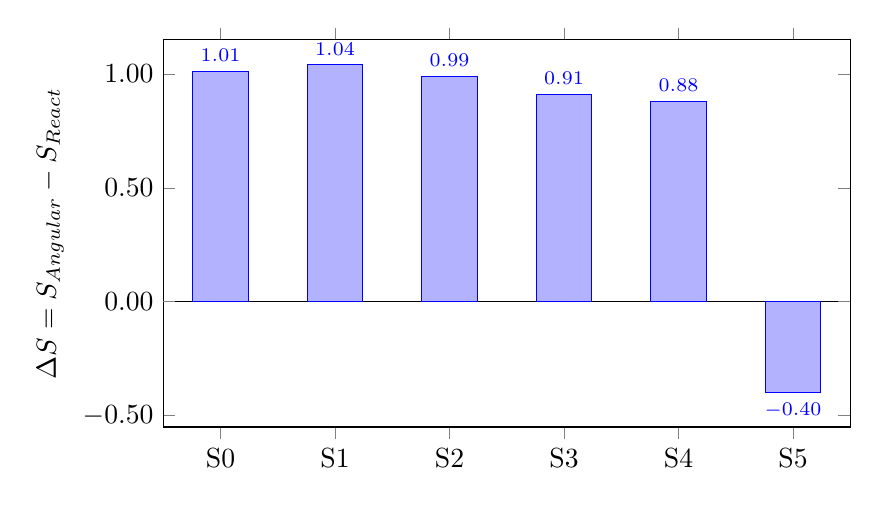
\begin{tikzpicture}
\begin{axis}[
  ybar, bar width=20pt,
  ymin=-0.55, ymax=1.15,
  symbolic x coords={S0,S1,S2,S3,S4,S5},
  xtick=data,
  ylabel={$\Delta S = S_{\text{Angular}} - S_{\text{React}}$},
  width=0.85\textwidth, height=6.5cm,
  enlarge x limits=0.1,
  nodes near coords,
  every node near coord/.append style={font=\scriptsize},
  /pgf/number format/.cd, fixed, zerofill, precision=2,
  extra y ticks=0,
  extra y tick labels=,
  extra y tick style={grid=major, major grid style={black}},
]
\addplot coordinates {(S0,1.01) (S1,1.04) (S2,0.99) (S3,0.91) (S4,0.88) (S5,-0.40)};
\end{axis}
\end{tikzpicture}
\caption{Brecha de puntuación entre Angular y React en los seis escenarios. Valores positivos
indican preferencia por Angular. S5 (límite hipotético que ignora seguridad y cumplimiento) es
el único escenario en que React resulta superior ($\Delta S = -0.40$).}
\label{fig:4.4}
\end{figure}

En los cinco escenarios compatibles con un entorno bancario regulado
(S0--S4), Angular mantiene la preferencia con márgenes entre 0.88 y 1.04
puntos. El contraste entre S0 (con criterios de IA, $\Delta S = 1.01$) y S3
(sin criterios de IA, $\Delta S = 0.91$) es la evidencia empírica central
para la Hipótesis Específica 6: incorporar los criterios asociados a la IA
generativa \emph{amplía} la ventaja de Angular en 0.10 puntos, en lugar de
introducir una fuente de incertidumbre --lo que confirma que la calidad y
gobernanza del código IA-asistido no son un factor neutro, sino que
refuerzan la preferencia por frameworks tipados y opinionados. Un segundo
hallazgo relevante es que, al haber retirado del modelo los criterios
organizacionales (ecosistema y talento) que en la versión previa de esta
metodología constituían la principal fortaleza relativa de React, ningún
escenario compatible con la regulación bancaria logra revertir la decisión:
solo el escenario S5 --que ignora por completo la seguridad y el
cumplimiento normativo, y que ninguna institución financiera regulada
podría adoptar-- favorece a React. Esta mayor robustez frente al modelo de
cuatro dimensiones evaluado en una versión anterior de la metodología
constituye, en sí misma, evidencia de que centrar el modelo en los ejes
técnico y regulatorio --tal como establece el título de esta
investigación-- produce una decisión tecnológica más estable ante la
incertidumbre en la ponderación de expertos.
